\chapter{Question2}
\section{问题概述}
%
%%对问题的直观描述
%
本问题要求利用神经网络拟合$[-2\pi,2\pi]$范围内的正弦函数。

%
%对项目已有代码的阅读和理解
%

%
%解决问题的思路和想法
%

\section{算法设计}
%
%用自己的语言描述解决问题所使用的算法的原理及功能,设计思路和算法流程图
%
理论上,二层神经网络便能以任意精度拟合任何给定的连续函数。对于本问题,只需要拟合$[-2\pi,2\pi]$范围内的正弦函数,因此二层神经网络就足够了。
最终我使用的神经网络架构为:
\begin{center}
    输入$\rightarrow$线性层$\rightarrow$非线性层$\rightarrow$线性层$\rightarrow$输出
\end{center}
其中,线性层中包含偏置值,非线性层为使用ReLU函数。

在训练的过程中,我依据模型在当前批次样例上的损失函数值来判断是否应当结束训练。
\section{算法实现}
%
%在算法原理的基础上,结合代码,讲述算法的实现细节、核心函数、模块输入输出,数据结构定义等内容
%

\begin{lstlisting}[emph={[3]dataset,x,y},emphstyle={[3]\color{vscode_parametercolor}},emph={[4]RegressionModel,GameState,MinimaxAgent,AlphaBetaAgent},emphstyle={[4]\color{vscode_classcolor}}]
class RegressionModel(object):
    def __init__(self):
        self.layer_size = 512
        self.feature_num = 1
        self.output_num = 1
        self.learning_rate = 0.05
        self.batch_size = 200
        self.threshold = 0.01
        self.w1 = nn.Parameter(self.feature_num,self.layer_size)
        self.b1 = nn.Parameter(1,self.layer_size)
        self.w2 = nn.Parameter(self.layer_size,self.output_num)
        self.b2 = nn.Parameter(1,self.output_num)
        self.W = [self.w1,self.b1,self.w2,self.b2]

    def run(self, x):
        return nn.AddBias( nn.Linear( nn.ReLU( nn.AddBias( nn.Linear(x,self.w1),self.b1)),self.w2),self.b2)

    def get_loss(self, x, y):
        return nn.SquareLoss(self.run(x),y)

    def train(self, dataset):
        for x,y in dataset.iterate_forever(self.batch_size):
            gradients = nn.gradients(self.get_loss(x,y),self.W)
            for i,w in enumerate(self.W):
                w.update(gradients[i],-self.learning_rate)
            loss = self.get_loss(x,y)
            if nn.as_scalar(loss) <= self.threshold:
                break

\end{lstlisting}

%
\section{实验结果}
我成功获得了本问题的所有分数。本问的评分依据便是训练好的神经网络在测试集上得到的损失函数值。
\begin{figure}[htbp]
    \centering
    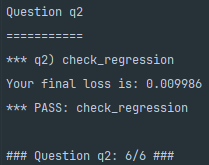
\includegraphics{pic/q2.png}
    \caption{Question2实验结果}\label{q2}
\end{figure}
%
%实验中遇到的问题及解决方案,收获和思考:对算法的理解、优缺点的评价、算法的适用场景
%
